%Chapter 3

\renewcommand{\thechapter}{3}

\newcommand{\swave}[0]{$\it{s}$-wave}
\newcommand{\pwave}[0]{$\it{p}$-wave}
\newcommand{\K}{$^{40}\rm{K}$}
\newcommand{\Rb}{$^{87}\rm{Rb}$}
\newcommand{\us}{$\rm{\mu s}$}
\newcommand{\mT}{$\rm{mT}$}
\newcommand{\ez}{$\mathit{\bf{e_z}}$}
\newcommand{\ex}{$\mathit{\bf{e_x}}$}
\newcommand{\um}{$\rm{\mu m}$}
\renewcommand{\thefootnote}{\arabic{footnote}}



\chapter{Direct measurement of a Feshbach resonance in \K{} via observation of \it{s}-wave scattering}

\section{Introduction}
Feshbach resonances are widely used for tuning the interaction strength in ultracold atomic gases. They have been particularly instrumental in the study of interactions and interaction-dependent processes in cold Fermi gases. In contrast to atomic Bose-Einstein condensates (BECs), where even weak interactions play a crucial role, for example giving rise to their characteristic Thomas-Fermi density profiles \cite{KetterleBEC},  interractions must compete with the Fermi energy before becoming relevant. Practically speaking, the density of Fermi clouds is typically $\sim$1000 times less than that of BECs \footnote{This is not the case for recently realized erbium and dysprosium DFGs \cite{Aikawa14,Lu12}, where strong dipolar interactions are present.}, making it necessary to enhance the strength of interactions in order to observe significant interaction effects\cite{KetterleDFG}. The tunability of interactions provided by Feshbach resonances has allowed for creation of molecular Bose-Einstein condensates from Fermi gases \cite{Greiner03,Zwierlein03, Jochim03} as well as observation of the phase transition from the Bardeen-Cooper-Schrieffer (BCS) superconduting regime to the BEC regime at sufficiently low temperatures \cite{Bartenstein04, Bourdel04, Zwierlein04, Regal04}.
\par A Feshbach resonance occurs when a diatomic molecular state energetically approaches the two-atom continuum \cite{Chin10, Timmermans99}. In experiment, the relative energy of the free atomic states in two hyperfine sublevels and the molecular state is defined by a bias magnetic field. Consequently, the Feshbach resonance can be accessed by changing the bias field. In the simple case where there are no inelastic two-body channels, such as for the \K{} resonance discussed in this work, the effect of the resonance on the scattering length between two free atoms is \cite{Chin10}
\begin{equation}
a(B)=a_{\rm{bg}}\left(1-\frac{\Delta}{B-B_0}\right),
\label{feshbachEq}
\end{equation}
where $a_{\rm{bg}}$ is the background scattering length, $\Delta$ is the width of the resonance, and $B_0$ is the field value at which the resonance occurs. The scattering length diverges at the resonance.
\par  The exact value of the resonant field $B_0$ is difficult to calculate analytically and is commonly computed via numerical models based on experimental input parameters \cite{Tiesinga93, Lysebo09, Gao11} or determined experimentally \cite{Inouye98, Cornish00}. Many experimental techniques have been used to characterize Feshbach resonances, including the observation of atom loss due to three-body inelastic scattering, measurement of re-thermalization timescales, and anisotropic expansion of the cloud upon release from a confining potential, all of which infer the elastic scattering cross section from collective behavior of the cloud \cite{Regal03,OHara02,Monroe93}.
\par Here we used direct scattering as a primary probe of the location and width of a Feshbach resonance. We collided pairs of ultra-cold Fermi gases and directly imaged the resulting \swave{} scattered atoms as a function of magnetic field strength. This allowed us to observe the enhancement in scattering without relying on proxy effects. We measured the fraction of atoms scattered during the collision, and from this fraction deduced the resonant magnetic field  and the width of the resonance.
%A similar technique has been used to characterize impurity scattering in BECs \cite{Chikkatur00}.
%\par The techniques developed in this experiment for observing Fermion scattering can be extended to engineering higher order partial wave interactions, as has been done for bosons \cite{Williams2012}.

In our dilute DFGs, even with the resonant enhancement of the scattering cross section, only a small fraction of the atoms scattered as the clouds passed through each other. This made direct detection of scattered atoms difficult due to detection uncertainty that disproportionately affected regions of low atomic density. To optimize the signal-to-noise ratio (SNR) for low atom numbers, we absorption imaged with fairly long, high-intensity pulses --- a non-standard regime, where the atoms acquired a velocity during imaging and the resulting Doppler-shift was non-negligible.  Simulation of the absorption imaging process was necessary for an accurate interpretation of these images. Using the simulation-corrected images, we extracted the fraction of atoms scattered in our collision experiment.

This paper is divided into two parts. In the first, we study absorption imaging in the presence of a significant time-dependent Doppler shift and show how we use our results to interpret data. In the second, we describe our \swave{} scattering experiment and extract a measure of the location and width of the Feshbach resonance in \K{}.

\section{Experimental setup}
In this section we describe our Fermi scattering experiment. We collided two counter-propagating \K{} clouds and observed the resulting \swave{} halo of scattered atoms.  We measured the dependence of the scattered atomic fraction on the bias magnetic field in the vicinity of the Feshbach resonance. We used this data to extract the location of the magnetic fields resonance of 20.206(15) \mT{} and a width of 1.0(5) \mT{}, similar to the accepted values of 20.210(7) \mT{} and 0.78(6) \mT{} \cite{Regal04}.

We prepared clouds of cold \K{} atoms in a hybrid \K{} and \Rb{} apparatus, previously described in \cite{Williams13, Lin09, KarinaThesis}. We used a Zeeman slower to slow both species before capturing in a magneto-optical trap (MOT). After 7 s seconds of MOT loading \K{} followed by 1.5 s of loading both \K{} and \Rb{}, we cooled both species in optical molasses for 2 ms. We optically pumped both species into their maximally stretched magnetically trappable states, $\ket{F=9/2, m_F=9/2}$ for \K{} and $\ket{F=2,m_F=2}$ for \Rb{}. Both species were then loaded into a quadrupole magnetic trap with a $\approx$ 7.68 mT/cm gradient along \ez, and cooled evaporatively via forced RF evaporation, sweeping the RF frequency from 18 MHz to 2 MHz in 10 s. The magnetic trap was plugged by a $\lambda =$ 532 nm beam, tightly focused to $\approx$ 30 \um{} and $\approx$ 5 W in power, providing a repulsive potential around the zero field point to prevent Majorana losses. Since the \K{} atoms were spin polarized and therefore only interacted by the strongly suppressed \pwave{} interactions, they re-thermalized only due to sympathetic cooling with \Rb{} atoms.

We then loaded the atoms into a crossed optical dipole trap, provided by a 1064 nm fiber laser, and continued evaporative cooling by slowly ramping down the dipole trap to trap frequencies of $(\omega_x,\omega_y,\omega_z)/2\pi =(39, 42, 124)$ Hz in the three spatial directions, while also turning off the quadrupole field. We then used adiabatic rapid passage (ARP) to transfer the \Rb{} atoms from the $\ket{F=2, m_F=2}$ state to the  $\ket{F=1, m_F=-1}$ absolute ground state via 6.8556 GHz microwave coupling (20.02 MHz from the zero field resonance) followed by a magnetic field sweep from -0.469 mT to -0.486 mT in 50 ms. This state was chosen to minimize spin changing collisions with \K{} atoms during any further evaporation \cite{BestThesis}.  We then briefly applied an on-resonant probe laser, ejecting any remaining \Rb{} atoms in the $F=2$ manifold from the trap. We again used ARP to transfer the \K{} atoms into the $\ket{F=9/2,m_F=-9/2}$ state by using a 3.3 MHz rf field and sweeping the bias magnetic field from -0.518 mT to -0.601 mT in 150 ms.

Following the state transfer, we had two versions of the protocol \--- one for approaching the Feshbach resonance from higher fields and one for approaching it from lower fields. For approaching the resonance from lower fields, we proceeded by ramping the bias magnetic field to 19.05 mT, turning on a 42.42 MHz RF field, and then sinusoidally modulating the bias field at 125 Hz for 0.5 s, with a 0.14 mT amplitude, decohering the \K{} state into an equal mixture of $\ket{F=9/2,m_F=-9/2}$ and $\ket{F=9/2,m_F=-7/2}$. For approaching the resonance from higher fields, the same was done at a bias field of 21.71 mT and an RF frequency of 112.3 MHz. The depolarization allowed the \K{} atoms to interact and re-thermalize, allowing us to further evaporate in the dipole trap \cite{DeMarco99}. Since \Rb{} is heavier than \K{}, we were able to evaporate the \K{} atoms past the point where \Rb{} atoms were no longer suspended against gravity and had been completely removed.  These hyperfine states of \K{} were then used to study their Feshbach resonance.
\par After evaporation, we ramped the bias field in a two-step fashion to the desired value $B$ near the Feshbach resonance. We approached the field using a large pair of  coils in Helmholtz configuration (0.19 mT/A) to bring the magnetic field to a setpoint 0.59 \mT{} away from $B$,  $B-0.59$ \mT{} when approaching from below and $B+0.59$  \mT{} from above. We held the atoms at this field for 100 $\rm{ms}$ to allow the eddy currents induced by the large coils to settle, and then used a lower inductance (0.017 mT/A) set of Helmholtz coils to quickly change the field the remaining 0.59 \mT{}. This allowed us to study the resonance from both sides without the added losses associated with going through the resonance \cite{Chin10}.

Once at the intended bias field, we split the cloud into two spatially overlapping components with opposing momenta  and observed scattering as they moved through each other and separated. These counterpropagating components were created using an  8$E_{\rm{L}}$ deep near resonant ($\lambda_{\rm{L}}$=766.704 nm) 1-d retro-reflected optical lattice, where $E_{\rm{L}}=\hbar^2 k_{\rm{L}}^2/2m_{\rm{K}}$ is the lattice recoil energy and $\hbar k_{\rm{L}}=2\pi \hbar/ \lambda$ is the recoil momentum. We rapidly pulsed this lattice on and off with a double-pulse protocol \cite{Wu05, Edwards10}. The pulse sequence was optimized to transfer most of the atoms into the $\pm 2 \hbar k_{\rm{L}}$ momentum states. Since the initial Fermi gas had a wide momentum spread (in contrast to a BEC, which has a very narrow momentum spread), and the lattice pulsing is a momentum dependent process  \cite{Wu05}, not all the atoms were transferred into the target momentum states. We optimized our pulse times to minimize the atoms remaining in the zero momentum state. The optimized pulse times were 23 \us{} for the first pulse, 13 \us{} off interval, and 12 \us{} for the second pulse \cite{Edwards10}.

We then released the atoms from the trap and allowed 1 ms for the two opposite momentum states within the cloud to pass through each other, scattering on the way. For the data taken coming from below the Feshbach resonance, we then simply ramped down the field and imaged the atoms. For the data taken coming from above the Feshbach resonance, we ramped the field back up, retreating through the resonance if it had been crossed and thereby dissociating any molecules that were created, and then quickly ramped the field back down and imaged the atoms. We used a 40 \us{} imaging pulse with $I_0/I_{\rm{sat}}\approx 0.6$ at the center of the probe laser.

The total time-of-flight, the time from the moment the atoms were released from the trap to when they were imaged, was $t_{TOF}=6.8$ $\rm{ms}$. In such an image, the observed atomic position is determined by the initial velocity upon release from the trap, along with the time-of-fligt time $t_{TOF}$. Therefore, this technique measures the momentum and not the position distribution of the atoms.

The magnetic fields produced by our coils in the regime of interest were independently calibrated by rf-spectroscopy. We prepared \K{} atoms in the $\ket{F=9/2, m_F=-9/2}$ state and illuminated them with and rf-field with some frequency $\nu_{rf}$. We then ramped our high-inductance coils to variable set points, followed by an adiabatic 250\us{} ramp of 2.84 mT in the lower inductance coils. We then used Stern-Gerlach and observed the fractional population in the $\ket{F=9/2, m_F=-9/2}$  and $\ket{F=9/2, m_F=-7/2}$ states as a function of the high-inductance coil current. We fit the fractional population curve to a Gaussian, and considered the center of the fit to be on-resonant, with an uncertainty given by the Gaussian width. We used the Breit-Rabi formula to determine the resonant field value at $\nu_{rf}$. We did this for 5 different rf frequencies, and acquired a field calibration with an uncertainty of 0.3 mT, which was included in the listed uncertainty on the center field of the Feshbach resonance.


\section{Methods}

We first processed each image by comparing the obsereved $OD$s to simulations taking into account the recoil induced detuning as described in Sec. \ref{sec:2}. An example of images before and after processing are shown in Fig. \ref{fig:SampleCorrection}.  To improve the signal and mitigate our shot to shot number fluctuations, we took 15 nominally identical images for each data point.
\begin{figure}
	\subfigure[]{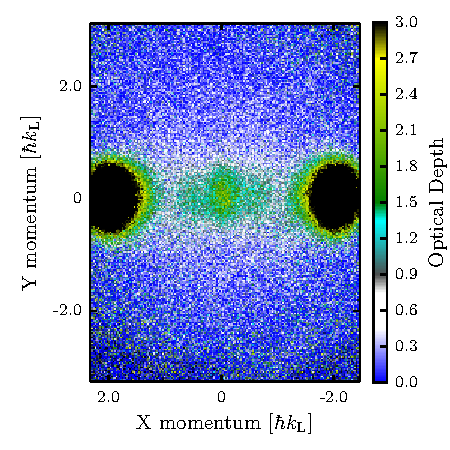
\includegraphics{Chapter3 Figures/figure10a.pdf}}
	\subfigure[]{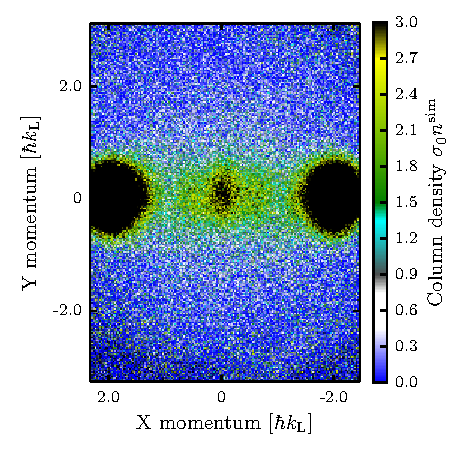
\includegraphics{Chapter3 Figures/figure10b.pdf}}
\caption{An example of our absorption image after 6.8 ms TOF. The 1-D lattice imparts momentum along \ex{}. The two large clouds on the left and right are the atoms in the $\pm 2 k_{\rm{L}}$ momentum orders that passed through each other unscattered. The smaller cloud in the center is the atoms that remained in the lowest band of the lattice after pulsing, and thus obtained no momentum. The thin spread of atoms around these clouds is the atoms that underwent scattering.   This image was taken coming from below the Feshbach resonance at 20.07  \mT{}. (a) Raw optical depth, (b) atomic column density obtained by comparing to simulated $OD$s, $\sigma_0 n^{\rm{sim}}$ }
\label{fig:SampleCorrection}
\end{figure}

We counted the fraction of atoms that experienced a single scattering event for each of the fifteen images at a given bias magnetic field. Single scattering events are easily identified, as two atoms that scatter elastically keep the same amplitude of momentum, but depart along an arbitrary direction. Therefore, an atom traveling at $2 \hbar k_{\rm{L}}$ to the right that collides elastically with an atom traveling at $-2 \hbar k_{\rm{L}}$ to the left will depart with equal and opposite momenta $2 \hbar k_{\rm{L}}$ at an arbitrary angle, and in a time of flight image such atoms will lie in a spherical shell, producing the scattering halo pictured in Fig. \ref{fig:halo}(a).
\begin{figure}
	\subfigure[]{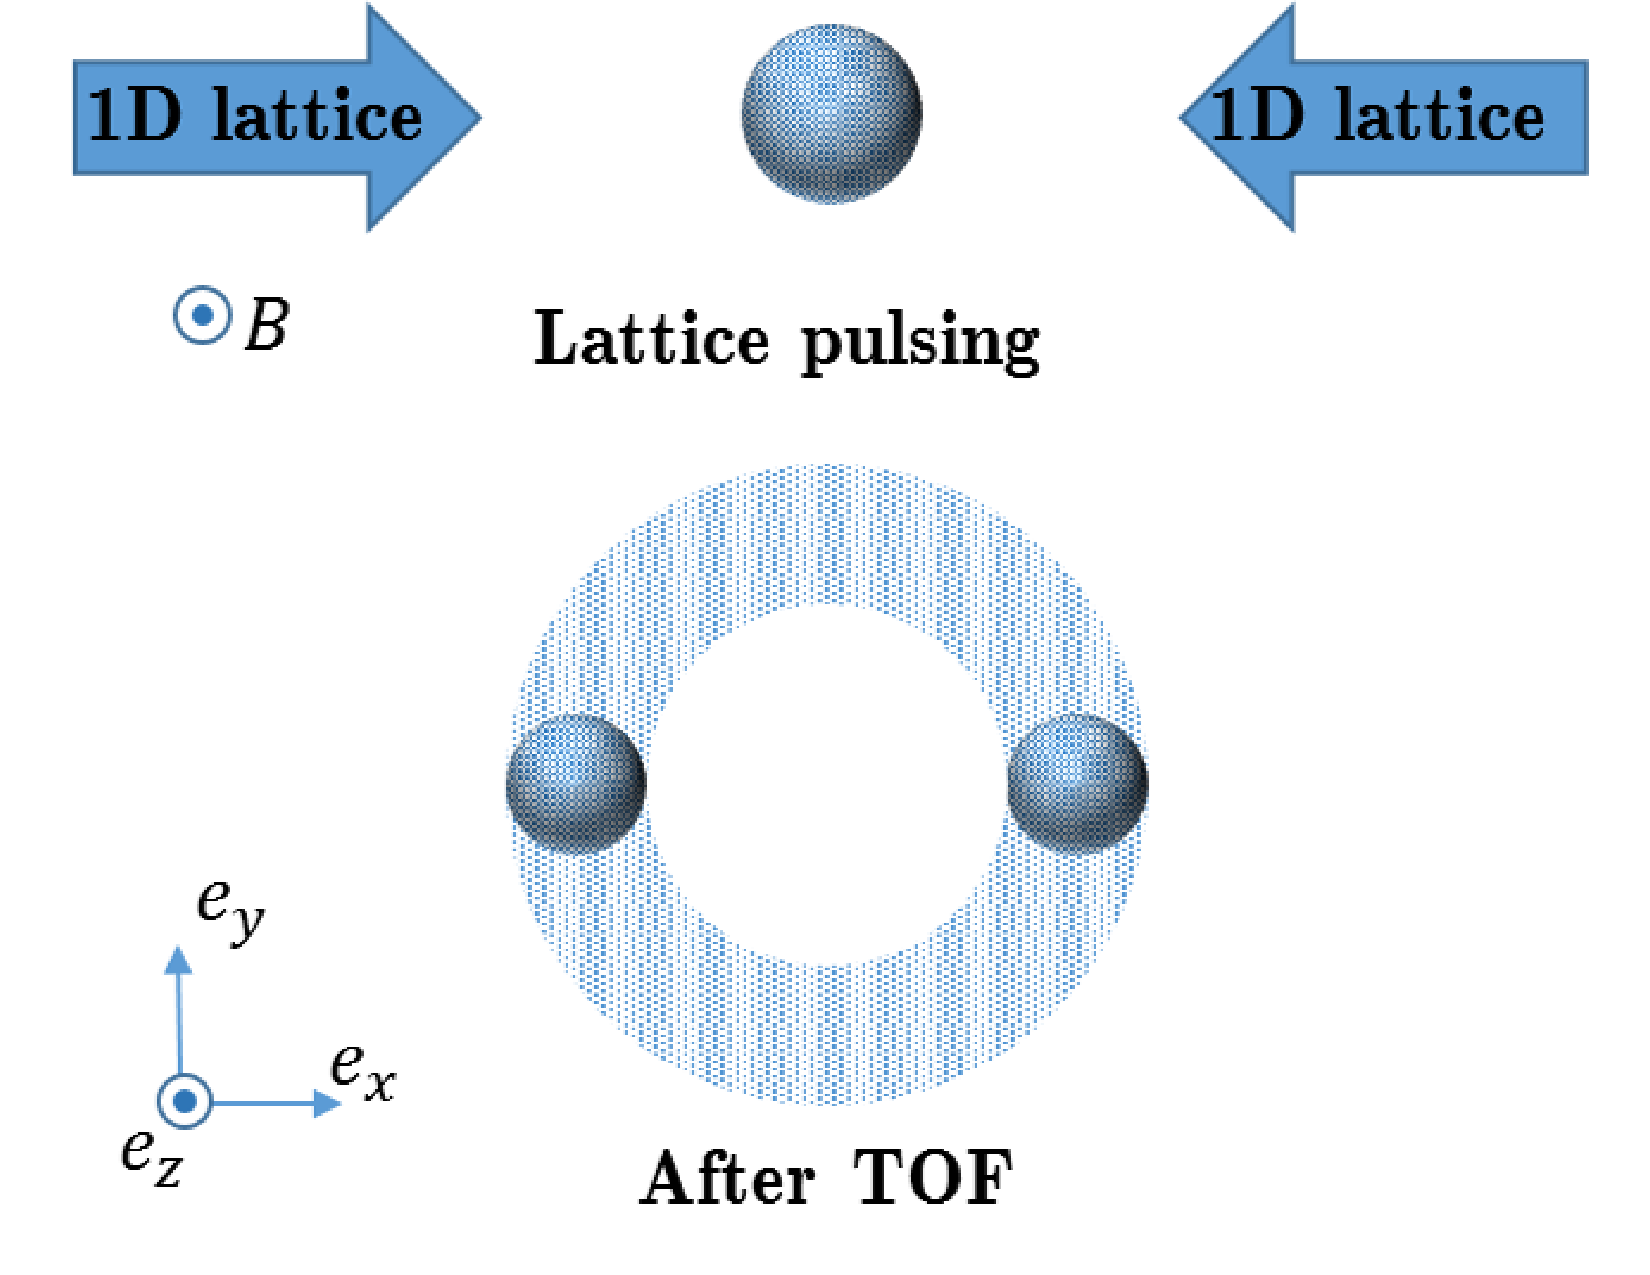
\includegraphics[scale=0.25]{Chapter3 Figures/Picture12.pdf}}
	\subfigure[]{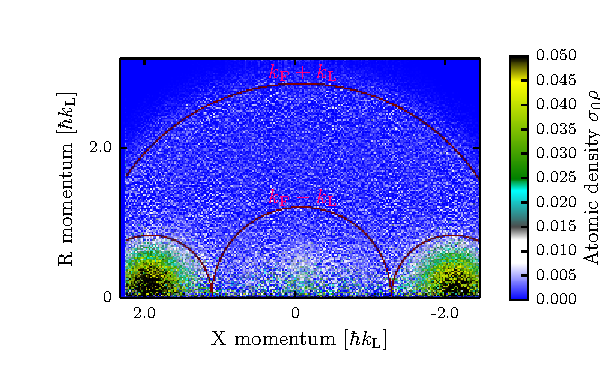
\includegraphics{Chapter3 Figures/figure12b.pdf}}
\caption{(a) Our experimental setup. After time of flight, the two clouds traveling along $\pm \hat{e}_x$ directions have separated and the atoms that underwent a single scattering event were evenly distributed in a scattering halo around the unscattered clouds. The 1-D lattice defined the axis of cylindrical symmetry. (b) Inverse Abel transformed image. The atoms within the Fermi momentum $k_F$ of each unscattered cloud center are in the unscattered region and counted towards the total unscattered number. The atoms outside the radius $ k_{\rm{L}}-k_{\rm{F}}$ but inside $k_{\rm{L}}+k_{\rm{F}}$ but outside the unscattered region are counted towards the number of single scattered atoms.   }
\label{fig:halo}
\end{figure}

Absorption images captured the integrated column density along \ez{}, a projected 2D atomic distribution. To extract the radial dependence of the 3D distribution from the 2D image, we performed a standard inverse Abel transform. The inverse Abel transform assumes cylindrical symmetry, which was present in our case, with the axis of symmetry along \ex{}, defined by the lattice. We neglect the initial asymmetry of the trap, as during time-of-flight the atoms travel far beyond the initial extent of the cloud  $(r_x,r_y,r_z)\approx$ (45,48,15) \um{}, while the cloud width after TOF is $\approx$ 82 \um in each direction. We thus obtained the atomic distribution $\rho(r,\theta)$ as a function of $r$, the radial distance from the scattering center, and $\theta$, the angle between $r$ and symmetry axis \ex{}, integrated over $\phi$, the azimuthal angle around the $x$ axis.

We then extracted the number of scattered atoms $N_{\rm{scat}}$ as a fraction of the total atom number $N_{\rm{tot}}$ for each image, as shown in Fig. \ref{fig:halo}(b). The unscattered atom number was the number of atoms in the two unscattered clouds. The number of atoms that underwent a single scattering event was the number of atoms outside the Fermi radius of the unscattered clouds, but inside the arc created by rotating the Fermi momentum $k_{\rm{F}}$ around the original center of the cloud (red arcs in Fig. \ref{fig:halo}(b)). For both the scattered and unscattered numbers, we accounted for atoms that fell outside the field of view of our camera by multiplying the counted atom number by a factor of the total area as defined by the radii divided by the visible area on the camera. The atoms in the center region were not counted as they were originally in the zero momentum state and could not contribute to the scattering halo under study.

We fit the fraction of scattered atoms versus the total atom number for each of the 15 images taken at the same bias magnetic field to a line constrained to be zero at zero. The slope of this fit was taken to be the value of $N_{\rm{scat}}/N_{\rm{tot}}^2$ at that bias magnetic field, and the variance of the fit gave the uncertainty on that data point. This uncertainty reflected our shot to shot number fluctuations, which produced variable atomic densities and thus influence the scattered fraction. 

We then deduced the resonant field value $B_0$ and width of the resonance  $\Delta$, the parameters in Eq. (\ref{feshbachEq}).  Since we were in the low energy regime (the atomic momentum was much smaller than the momentum set by the van der Waals length $k_{\rm{L}}+k_{\rm{F}}\ll1/l_{\rm{vdW}}$, and we were well below the p-wave threshold temperature \cite{DeMarco99}), the scattering cross-section was given by $\sigma=4\pi a^2$.

The scattering cross-section $\sigma$ gives the probability $P_{\rm{scat}}=\sigma N/A$ that a single particle will scatter when incident on a cloud of atoms with a surface density of $N/A$, where $A$ is the cross-sectional area of the cloud and $N$ is the number of atoms in the cloud. In our case, each half of the initial cloud, with atoms number $N_{\rm{tot}}/2$, is incident on the other half. Thus, the number of expected scattering events is $N_{\rm{scat}}= (N_{\rm{tot}}/2) \sigma  (N_{\rm{tot}}/2)=\sigma N_{\rm{tot}}^2/4A$. Assuming $A$ is constant for all our data, we can define a fit parameter $b_0=4\pi a_{\rm{bg}}^2/4A$, where $a_{\rm{bg}}$ is the background scattering length. We can thus adapt Eq. (\ref{feshbachEq}) to obtain the fit function
\begin{equation}
\frac{N_{\rm{scat}}}{N_{\rm{tot}}^2}=b_0\left(1-\frac{\Delta}{B-B_0}\right)^2 + C.
\label{eq:fit}
\end{equation}
We found that our imaging noise skewed towards the positive, giving rise to a small background offset. We accounted for this in our fit by including a constant offset parameter $C$.


\section{Results}
Our final data is presented in Fig. \ref{fig:fittedFractions}. The red curve depicts a best fit of the model given in Eq. (\ref{eq:fit}). The fit parameters we extracted were $\Delta = 1(5)$  \mT{}, $B_0 = 20.206(15)$  \mT{}, $b_0 = 5(3)\times 10^{-3}$ and $C=8(1)\times 10^{-4}$. To obtain the fit, we used data taken by approaching the resonance from above for points above where we expected the resonance to be and data taken approaching the resonance from below for points below. We also excluded from the fit data points very near the resonance, as there the assumption $\sigma\rho\ll1$, where $\rho$ is the atom number per unit area, is no longer valid and the problem must be treated hydrodynamically.

The accepted values for the $^{40}K$ s-wave Feshbach resonance for the  $\ket{9/2,-9/2}$ and $\ket{9/2,-7/2}$ states are $B_0=20.210(7)$  \mT{} and $\Delta=0.78(6)$  \mT{} \cite{Regal04}, which is in good agreement with our findings. Some potential sources of systematic uncertainty that we did not account for include scattering with atoms that did not receive a momentum kick from the lattice pulsing or the impact of multiple scattering events.
\begin{figure}
	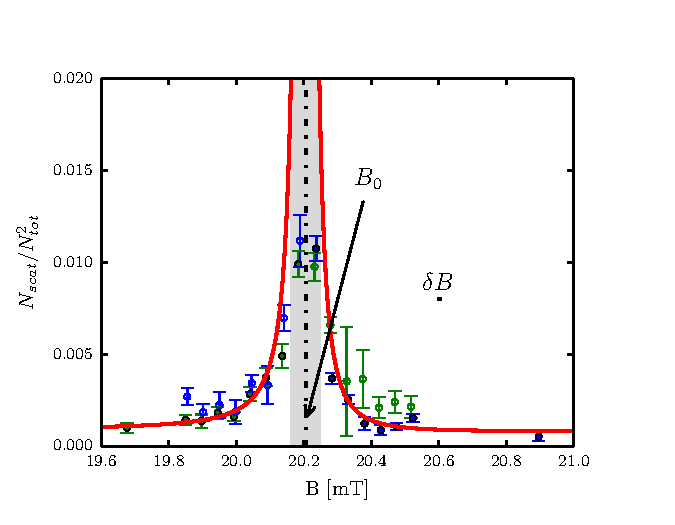
\includegraphics{Chapter3 Figures/figure11.pdf}
\caption{Normalized scattered population plotted versus bias field $B$. Green dots represent data taken coming from below the resonance, and blue dots represent the data taken coming from above the resonance. The red curve depicts the best fit, where data coming from above the resonance was used above the resonance and data coming from below the resonance was used below the resonance to create the fit; the unused data points are indicated by hollow dots. The regime where the scattering length is likely large enough for the atoms to behave hydrodynamically is shaded in gray, and data points in that area were also excluded from the fit. Resonant field value $B_0$ as found in this work and our systematic uncertainty in the bias magnetic field $\delta B_0$ are indicated.    }
\label{fig:fittedFractions}
\end{figure}
\section{Conclusion}
We studied the effects of recoil-induced detuning effects on absorption images and found an optimal imaging time of $\approx40$ \us{} for \K{} atoms for noise minimization after corrections. We use these results to observe s-wave scattering halos of the Fermi gas around the $\approx 20.2$ \mT{} Feshbach resonance and directly verified the resonance location and width. Our analysis can be used in any absorption imaging application where SNR optimization is critical.

